\documentclass[11pt,a4paper]{report}

%\usepackage{blindtext,expdlist}
\usepackage{styles/tumlogo}
%\usepackage[dvips]{graphicx}
\usepackage[pdftex]{graphicx}
 \DeclareGraphicsExtensions{.jpg,.JPG,.png,.pdf,.eps}
 \graphicspath{{figures/}} 
\usepackage[english]{babel}
\usepackage{amsmath}
\usepackage{amssymb}
\usepackage{listings}
\usepackage{color}

\definecolor{mygreen}{rgb}{0,0.6,0}
\definecolor{mygray}{rgb}{0.5,0.5,0.5}
\definecolor{mymauve}{rgb}{0.58,0,0.82}

\lstset{ %
  backgroundcolor=\color{white},   % choose the background color; you must add \usepackage{color} or \usepackage{xcolor}
  breakatwhitespace=false,         % sets if automatic breaks should only happen at whitespace
  breaklines=true,                 % sets automatic line breaking
  captionpos=b,                    % sets the caption-position to bottom
  commentstyle=\color{mygreen},    % comment style
  deletekeywords={...},            % if you want to delete keywords from the given language
  keepspaces=true,                 % keeps spaces in text, useful for keeping indentation of code (possibly needs columns=flexible)
  keywordstyle=\color{blue},       % keyword style
  language=C++,                    % the language of the code
  morekeywords={*,...},            % if you want to add more keywords to the set
  numbers=left,                    % where to put the line-numbers; possible values are (none, left, right)
  numbersep=5pt,                   % how far the line-numbers are from the code
  numberstyle=\color{mygray},      % the style that is used for the line-numbers
  rulecolor=\color{black},         % if not set, the frame-color may be changed on line-breaks within not-black text (e.g. comments (green here))
  showspaces=false,                % show spaces everywhere adding particular underscores; it overrides 'showstringspaces'
  showstringspaces=false,          % underline spaces within strings only
  showtabs=false,                  % show tabs within strings adding particular underscores
  stepnumber=1,                    % the step between two line-numbers. If it's 1, each line will be numbered
  stringstyle=\color{mymauve},     % string literal style
  tabsize=2,                       % sets default tabsize to 2 spaces
  title=\lstname                   % show the filename of files included with \lstinputlisting; also try caption instead of title
}

% Set here the title, authors and other stuff to be used for the cover
% This file is used by MAIN.TEX

% set title, authors and stuff for the cover
\def\doctype{Practical Course Report}

\def\title{HW/SW co-design with a LEGO car}
\def\subtitle{Car2X Communication}


\def\author{Hagen Schmidtchen, Paul Bergmann,\\ Johannes Windelen, Florian Janssen}
\def\date{August 15, 2014}

% text to appear in the footer
\def\footertext{}

%% Included by MAIN.TEX

% DEFINE NEW COMMANDS	
%\newcommand{\comments}[1]{}
%\newcommand{\mof}{\ac{MOF} }
%\newcommand{\omg}{\ac{OMG} }
%\newcommand{\uml}{\ac{UML} }
%\newcommand{\emf}{\ac{EMF} }
%\newcommand{\ecore}{\ac{Ecore} }

%\newcommand{\af}{Auto\textsc{FOCUS}~3 }

%\newcommand{\para}[1]{\vspace{-6mm}\paragraph{#1}}
%\newcommand{\seite}[1]{Chapter \ref{#1} on page \pageref{#1}}


% Defines the settings for the CAMP report document

%\renewcommand{\sectfont}{\normalfont \bfseries }        % Schriftart der Kopfzeile

% manipulate footer

%\usepackage {scrpage2}
%\pagestyle{scrheadings}
%\ifoot[\footertext]{\footertext} % \footertext set in INFO.TEX
 

%\setkomafont{pagehead}{\normalfont\rmfamily}

%\setkomafont{pagenumber}{\normalfont\rmfamily}
%% allow sophisticated control structures
%\usepackage{ifthen}


% use Palatino as default font
%\usepackage{palatino}

%\usepackage{wrapfig}


% use sans serif
%\renewcommand{\familydefault}{\sfdefault}

% Eurozeichen
%\usepackage[right]{eurosym}

% enable special PostScript fonts
%\usepackage{pifont}

%to use the subfigures
%\usepackage{subfigure}


%\usepackage{colortbl}

%\usepackage{caption}


%% show program code\ldots
%\usepackage{verbatim}
%\usepackage{program}

%% enable TUM symbols on title page
\usepackage{styles/tumlogo}

% Zeilenabstand
%\linespread {1.2}


% Vierstellige Gliederungstiefe im Inhaltsverzeichnis
%\setcounter{tocdepth}{3}

% 4-stellige Nummerierung
%\setcounter{secnumdepth}{3}

%\usepackage{multirow}

%% use colors
%\usepackage{color}

%% make fancy math
\usepackage{amsmath}
\usepackage{amsfonts}
\usepackage{amssymb}
\usepackage{textcomp}
\usepackage{yhmath} % f�r die adots 
%% mark text as preliminary
%\usepackage[draft,german,scrtime]{prelim2e}

%% create an index
%\usepackage{makeidx}

% for the program environment
%\usepackage{float}

%% load german babel package for german abstract
%\usepackage[german,american]{babel}
\usepackage[english]{babel}
%\selectlanguage{english}

% use german characters as well
%\usepackage[latin1]{inputenc}       % allow Latin1 characters

% use initals dropped caps - doesn't work with PDF
%\usepackage{dropping}

%\Abk�rzungsverzeichnis
%\usepackage[nolist]{acronym}

%\usepackage{styles/shortoverview}
%----------------------------------------------------
%      Graphics and Hyperlinks
%----------------------------------------------------

%% check for pdfTeX
\ifx\pdftexversion\undefined
 %% use PostScript graphics
 \usepackage[dvips]{graphicx}
 \DeclareGraphicsExtensions{.eps,.epsi}
 \graphicspath{{figures/}{figures/review}} 
 %% allow rotations
 \usepackage{rotating}
 %% mark pages as draft copies
 %\usepackage[english,all,light]{draftcopy}
 %% use hypertex version of hyperref
 \usepackage[hypertex,hyperindex=false,colorlinks=false]{hyperref}
\else %% reduce output size \pdfcompresslevel=9
 %% declare pdfinfo
 %\pdfinfo { 
 %  /Title (my title) 
 %  /Creator (pdfLaTeX) 
 %  /Author (my name) 
 %  /Subject (my subject	) 
 %  /Keywords (my keywords)
 %}
 %% use pdf or jpg graphics
 \usepackage[pdftex]{graphicx}
 \DeclareGraphicsExtensions{.jpg,.JPG,.png,.pdf,.eps}
 \graphicspath{{figures/}} 
 
 %% Load float package, for enabling floating extensions
 %\usepackage{float}
 
 %% allow rotations
 \usepackage{rotating}
 %% use pdftex version of hyperref
 \usepackage[pdftex,colorlinks=true,linkcolor=black,citecolor=black,%
 anchorcolor=red,urlcolor=red,bookmarks=true,%
 bookmarksopen=true,bookmarksopenlevel=0,plainpages=false,%
 bookmarksnumbered=true,hyperindex=false,pdfstartview=%
 ]{hyperref}
%
%\usepackage[pdftex,colorlinks=false,linkcolor=red,citecolor=red,%
% anchorcolor=red,urlcolor=red,bookmarks=true,%
% bookmarksopen=true,bookmarksopenlevel=0,plainpages=false%
% bookmarksnumbered=true,hyperindex=false,pdfstartview=%
% ]{hyperref}
\fi





%% Fancy chapters
%\usepackage[Lenny]{fncychap}
%\usepackage[Glenn]{fncychap}
%\usepackage[Bjarne]{fncychap}

%\usepackage[avantgarde]{quotchap}

% set the bibliography style
%\bibliographystyle{styles/bauermaNum}
%\bibliographystyle{alpha}

\bibliographystyle{unsrt}

%% Commands to be used within the TUM report document
% Included by MAIN.TEX
% Please include your own cool commands here. 
% Be only sure to comment it sufficiently so others can use it.

%-------------------------------------------------------------
%                      Own Commands
%-------------------------------------------------------------

\DeclareMathOperator{\atan2}{atan2}

%-------------------------------------------------------------
% math stuff -------------------------------------------------

% nice R, N, C
\newcommand{\nat}{\mathbb{N}}
\newcommand{\real}{\mathbb{R}}
\newcommand{\compl}{\mathbb{C}}



% norm
\newcommand{\norm}[1]{\left\| #1 \right\|}

% un demi
\newcommand{\half}{\frac{1}{2}}

% parantheses
\newcommand{\parenth}[1]{ \left( #1 \right) }
\newcommand{\bracket}[1]{ \left[ #1 \right] }
\newcommand{\accolade}[1]{ \left\{ #1 \right\} }
%\newcommand{\angle}[1]{ \left\langle  #1 \right\rangle }

% partial derivative: %#1 function, #2 which variable
% simple / single line version
\newcommand{\pardevS}[2]{ \delta_{#1} f(#2) }
% fraction version
\newcommand{\pardevF}[2]{ \frac{\partial #1}{\partial #2} }

% render vectors: 3 and 4 dimensional
\newcommand{\veciii}[3]{\left[ \begin{array}[h]{c} #1 \\ #2 \\ #3	\end{array} \right]}
\newcommand{\veciv}[4]{\left[ \begin{array}[h]{c} #1 \\ #2 \\ #3 \\ #4	\end{array} \right]}

% render matrices: 3  dimensional (arguments in row first order)
\newcommand{\matiii}[9]{\left[ \begin{array}[h]{ccc} #1 & #2 & #3 \\ #4 & #5 & #6 \\ #7 & #8 & #9	\end{array} \right]}
%DOESN'T WORK,DON'T KNOW WHY \newcommand{\mativ}[16]{\left[ \begin{array}[h]{cccc} #1 & #2 & #3 & #4 \\ #5 & #6 & #7 & #8 \\ #9 & #10 & #11 & #12 \\ #13 & #14 & #15 & #16 \end{array} \right]}


%-------------------------------------------------------------
%-------------------------------------------------------------


%-------------------------------------------------------------
% some abreviations ------------------------------------------
\newcommand{\Reg}{$^{\textregistered}$}
\newcommand{\reg}{$^{\textregistered}$ }
\newcommand{\Tm}{\texttrademark}
\newcommand{\tm}{\texttrademark~}
\newcommand {\bsl} {$\backslash$}

%-------------------------------------------------------------
%-------------------------------------------------------------


%-------------------------------------------------------------
% formating --------------------------------------------------

% Theorem & Co environments and counters
\newtheorem{theorem}{Theorem}[chapter]
\newtheorem{lemma}[theorem]{Lemma}
\newtheorem{corollary}[theorem]{Corollary}
\newtheorem{remark}[theorem]{Remark}
\newtheorem{definition}[theorem]{Definition}
\newtheorem{equat}[theorem]{Equation}
\newtheorem{example}[theorem]{Example}
\newtheorem{algorithm}[theorem]{Algorithm}

% inserting figures
\newcommand{\insertfigure}[4]{ % Filename, Caption, Label, Width percent of textwidth
	\begin{figure}[htbp]
		\begin{center}
			\includegraphics[width=#4\textwidth]{#1}
		\end{center}
		\vspace{-0.4cm}
		\caption{#2}
		\label{#3}
	\end{figure}
}




% referecing figures

\newcommand{\refFigure}[1]{ %label
	figure \ref{#1}
}
\newcommand{\refChapter}[1]{ %label
	chapter \ref{#1}
}

\newcommand{\refSection}[1]{ %label
	section \ref{#1}
}

\newcommand{\refParagraph}[1]{ %label
	paragraph \ref{#1}
}

\newcommand{\refEquation}[1]{ %label
	equation \ref{#1}
}

\newcommand{\refTable}[1]{ %label
	table \ref{#1}
}




\newcommand{\rigidTransform}[2]
{
	${}^{#2}\!\mathbf{H}_{#1}$
}

%code, in typewriter
\newcommand{\code}[1]
 {\texttt{#1}}

% comment that appears on the border - very practical !!!
\newcommand{\comment}[1]{\marginpar{\raggedright \noindent \footnotesize {\sl #1} }}


\newcommand{\clearemptydoublepage}{%
  \ifthenelse{\boolean{@twoside}}{\newpage{\pagestyle{empty}\cleardoublepage}}%
  {\clearpage}}

%-------------------------------------------------------------
%-------------------------------------------------------------


\newcommand{\etAl}{\emph{et al.}\mbox{ }}

%\addtolength{\evensidemargin}{-12mm}

%\newboolean{makeAll}
%\setboolean{makeAll}{true}

\begin{document}

	%\frontmatter
	
	%\ifmakeAll

		


% correct BCOR - undo at the end !!!
%\def\bcorcor{0.15cm}
%\addtolength{\hoffset}{\bcorcor}

\thispagestyle{empty}

 \vspace{4cm}
\begin{center}
	       \oTUM{4cm}
	   
	   \vspace{5mm}     
	   \huge FAKULT{\"A}T F{\"U}R INFORMATIK\\ 
	   \vspace{0.5cm}
	 \large DER TECHNISCHEN UNIVERSIT{\"A}T M{\"U}NCHEN\\
    \vspace{1mm}
        
	\end{center}
		

\vspace{5mm}
\begin{center}

   \Large \doctype

  \vspace{10mm}
  
  \huge\bf \title \\%[3ex]
  
  \vspace{5mm}
  
  \large \subtitle
  
  \vspace{15mm}  
  
  \author
  
  \vspace{15mm}
  
  \begin{figure}[h!]
  \centering
   
\includegraphics[width=4cm]{styles/informat.png}
  \end{figure}
  
  \end{center}
  %\newpage
		
		%\clearemptydoublepage
		
	%\fi	
		
		\tableofcontents
		%\clearemptydoublepage
	
	%\mainmatter
	
	

	%\ifthenelse{\boolean{makeAll}}{
	
		\chapter{Introduction}


\section{Motivation}
Paul

\section{Problem description}
Paul

\section{Approach}
Paul

		
%		\clearemptydoublepage
			
		\chapter{Concept}

\section{Overview}
Johannes

\section{Hardware structure}
The hardware is design to allow an easy exchange of components and extensions. A FPGA is used as main computation unit. All components used by the car are connected to this central unit. The communication between the car's components uses ethernet. This is also used for car2x communication through a wiport. Every wheel is controlled by a single nano FPGA, which uses an UART-to-ethernet converter to communicate with the main FPGA. A schematic structure can be seen in figure \ref{HWconc}.
\begin{center}
\begin{figure}[h]
	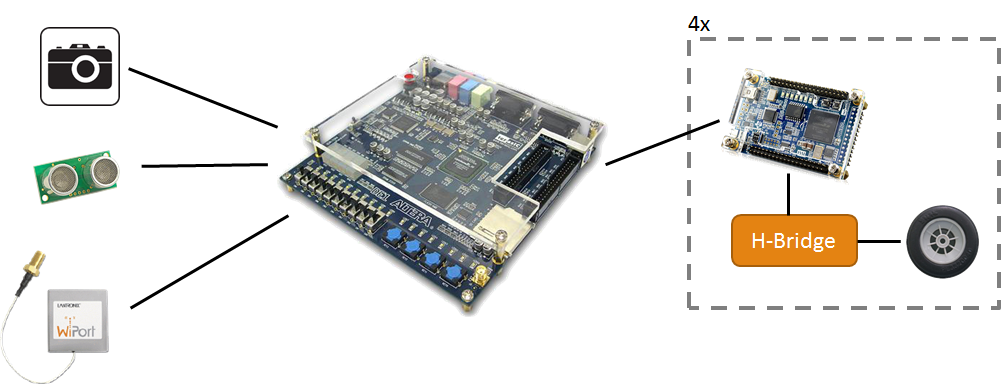
\includegraphics[width=\textwidth]{figures/hardwareconcept.png}
	\caption{Schematic hardware structure} \label{HWconc}
\end{figure}
\end{center}

\section{Communication Flow}
Paul - done

\section{Car2X Protocol}
The „CARP protocol"(developped by a previous lab-course group) was extended by a set of messages to let the NIOS2 processor system fit into the role of the communication central of the car. One NIOS2 core is handling the internal state of the car and the other one is in charge of all the communication between internal car parts and external communication partners like other cars or “car2x” stations. \newline
The internal communication protocol is based on the work of Florian Hisch and has nearly not been modified. The only major change was a role switch in terms of server-client relationship. Unlike before, the central unit now is a server to which external clients can connect to.
Keeping that in mind, there now is an external communication interface featuring the so called "Car2X-Messages" as an extension of the “CARP protocol”. Each message of this type, which is sent to the car, will be answered by the car after being processed or getting outdated. 
\newline
All this behaviour is handled on the "communication-core" of the NIOS2 system.
By parsing in the messages in the “socketserver.cpp” file directly from the incoming TCP/IP byte stream, there is a new message object created for every new message.
After that, the "sss exec command()" function handles the received message by reading out the message type an then taking various steps depending on the specific message.


		
%		\clearemptydoublepage
			
		\chapter{Hardware}
This chapter describes the basic concept and configuration of the car-system's hardware. A basic knowledge of Altera Quartus II is assumed.
\section{Topology}
Flo

\section{Configuration QSYS}
Flo

\section{Configuration Top Level File}
Flo

\section{Problems}
Flo

\section{WiPort}
Paul - done

\section{Circuit diagrams}
Johannes

		
%		\clearemptydoublepage
		
		\chapter{Software}

\section{Communication Core}

\section{CarControl Core}

\section{Shared memory Controller}

		
%		\clearemptydoublepage
		
		\chapter{Conclusion}
As the project goals were slightly changing over the lab course semester and the possible work and amount of ideas to be realized got into dimensions that could have filled many lab course semesters and not just one, we had to realize that we wont be able to build the perfect and completely stable Car2X platform without any bugs. We learned a lot of things aboout Software/Hardware co-design what includes a lot of time spent into looking for errors, bugs and hardware faults. This lead us to the decision to define our goal as getting the system far enough to run on our multicore FPGA and provide all the Car2X fatures in a way that it was possible to successfully test the functionalities in a way the positive results could be reproduced. This means that at the end we reached a state where the basic concept was successfully implemented and working BUT our result equals something comparable to an early developement prototype, meaning that there are definitely a lot of bugs and unhandeled cases making the car itself quite unstable in terms of reliability.\\ \\
Therefore we suggest to invest some decent amount of time into testing and optimizing the current state of the car because we sadly did not have the time to do that as well as we would have wanted to.
Also feel free to contact our group if you need some help. We know how hard it is to get into a previous' groups work...

		
%		\clearemptydoublepage
	
		
		%\part*{Anhang}		
		\appendix
		
		%\chapter{List of Symbols and Abbreviations}
\label{Anhang:Glossar}
\begin{tabbing}
	\hspace*{4cm} \= \kill  
	App \> Application --- usually for mobile devices \\[0.5ex]
\end{tabbing}
		
		
\section{Circuit diagrams} \label{appendix:circuits}

\begin{figure}[h]\label{appendix:pic_circuits_nano}
  \caption{The DE0 FPGA board pinout}
  \centering
    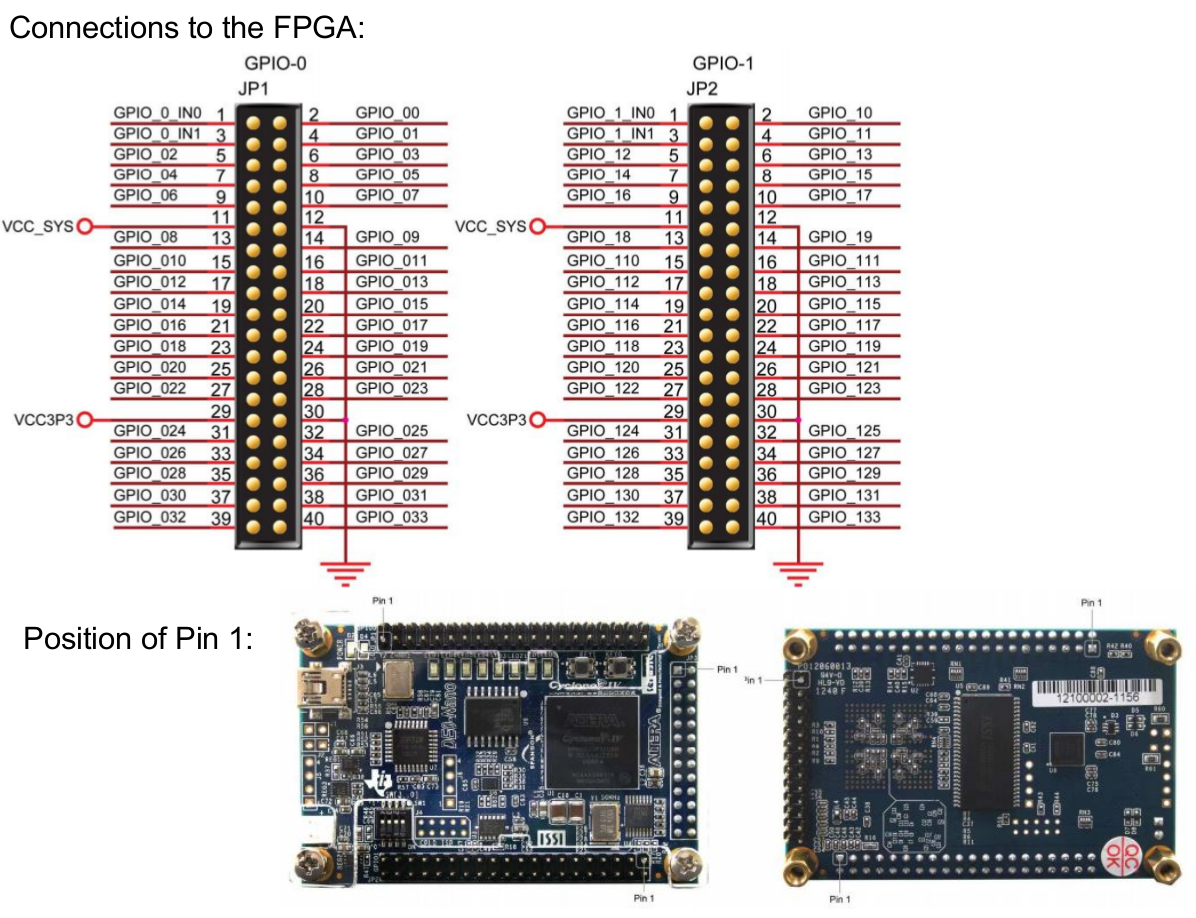
\includegraphics[width=1.0\textwidth]{figures/wiring_nano.png}
\end{figure}

\begin{figure}[h]\label{appendix:pic_circuits_nano_gpio0}
  \caption{The shared memory setup}
  \centering
    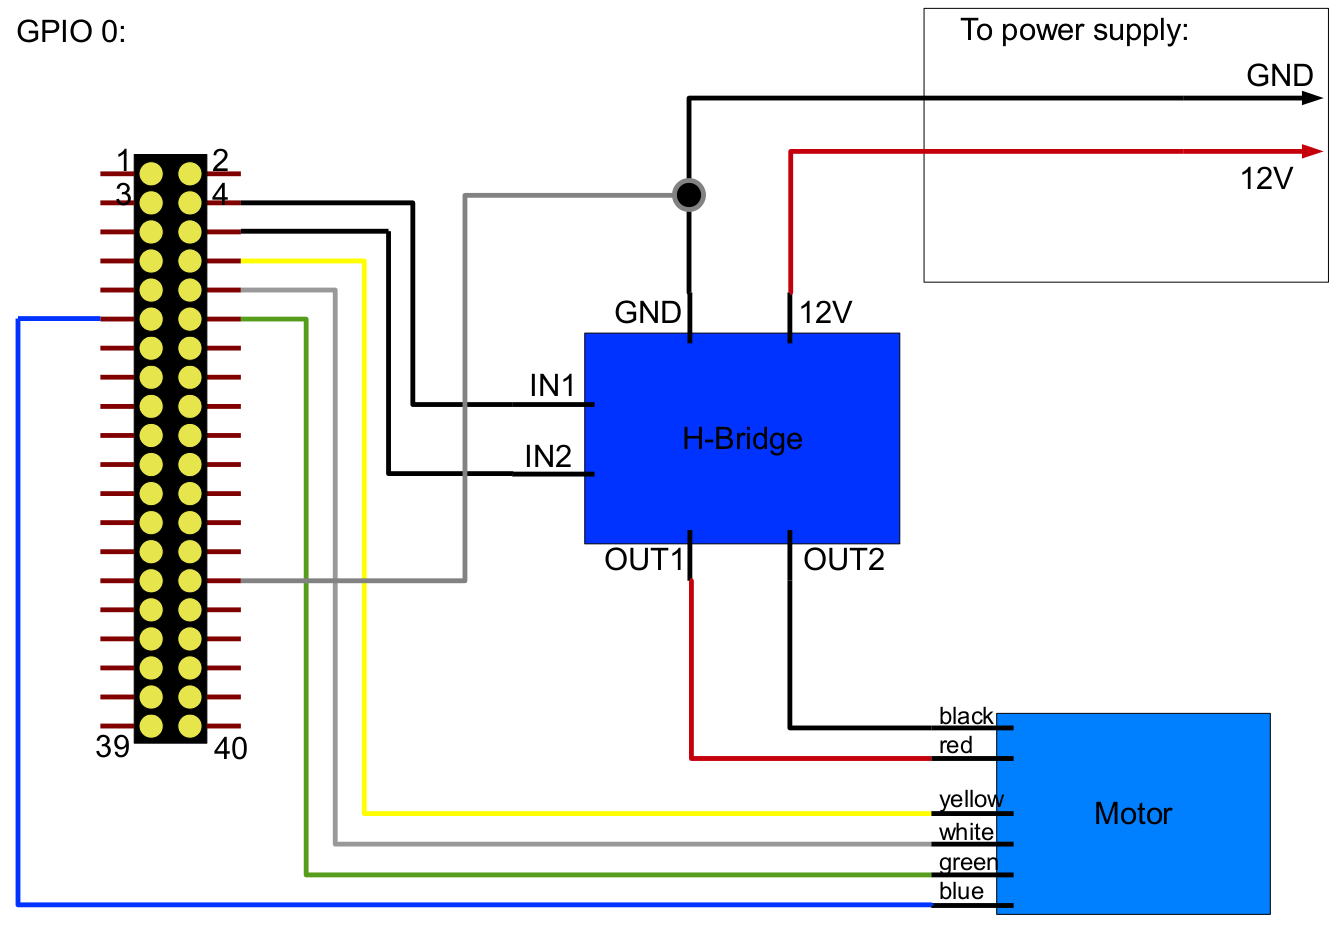
\includegraphics[width=1.0\textwidth]{figures/wiring_nano_gpio0.png}
\end{figure}

\begin{figure}[h]\label{appendix:pic_circuits_nano_gpio1}
  \caption{The shared memory setup}
  \centering
    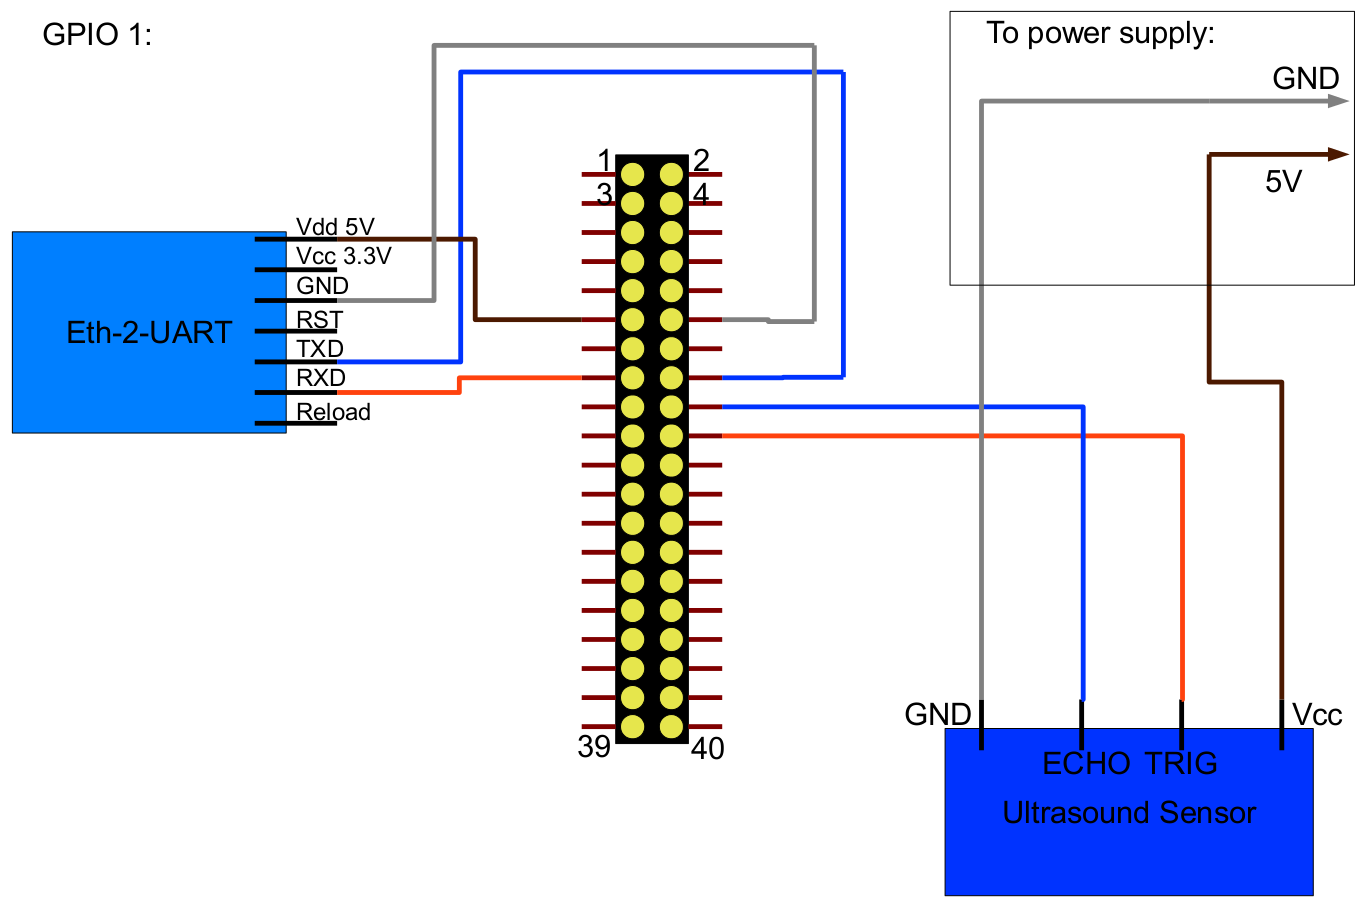
\includegraphics[width=1.0\textwidth]{figures/wiring_nano_gpio1.png}
\end{figure}

\begin{figure}[h]\label{appendix:pic_circuits_power_supply}
  \caption{The shared memory setup}
  \centering
    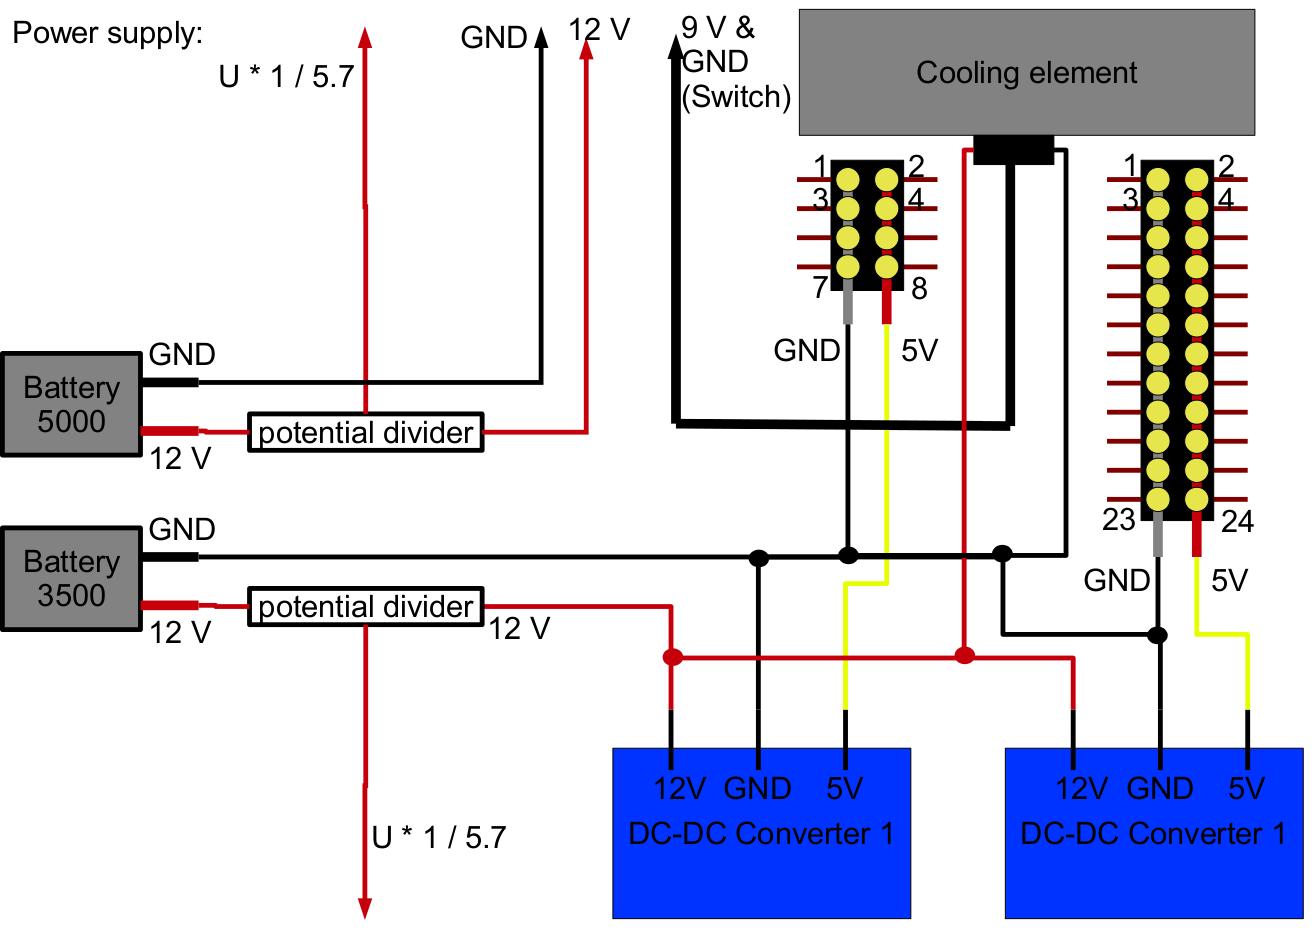
\includegraphics[width=1.0\textwidth]{figures/wiring_power_supply.png}
\end{figure}


		
		%\thispagestyle{empty}

		%\bibliography{Literatur/Referenzen}
		
	%}
	%{
	%}
		
		\raggedbottom
	
 
\end{document}
